% mnras_template.tex
%
% LaTeX template for creating an MNRAS paper
%
% v3.0 released 14 May 2015
% (version numbers match those of mnras.cls)
%
% Copyright (C) Royal Astronomical Society 2015
% Authors:
% Keith T. Smith (Royal Astronomical Society)

% Change log
%
% v3.0 May 2015
%    Renamed to match the new package name
%    Version number matches mnras.cls
%    A few minor tweaks to wording
% v1.0 September 2013
%    Beta testing only - never publicly released
%    First version: a simple (ish) template for creating an MNRAS paper

%%%%%%%%%%%%%%%%%%%%%%%%%%%%%%%%%%%%%%%%%%%%%%%%%%
% Basic setup. Most papers should leave these options alone.
\documentclass[a4paper,fleqn,usenatbib]{mnras}

% MNRAS is set in Times font. If you don't have this installed (most LaTeX
% installations will be fine) or prefer the old Computer Modern fonts, comment
% out the following line
\usepackage{newtxtext,newtxmath}
% Depending on your LaTeX fonts installation, you might get better results with one of these:
%\usepackage{mathptmx}
%\usepackage{txfonts}

% Use vector fonts, so it zooms properly in on-screen viewing software
% Don't change these lines unless you know what you are doing
\usepackage[T1]{fontenc}
\usepackage{ae,aecompl}


%%%%% AUTHORS - PLACE YOUR OWN PACKAGES HERE %%%%%

% Only include extra packages if you really need them. Common packages are:
\usepackage{graphicx}	% Including figure files
\usepackage{amsmath}	% Advanced maths commands
\usepackage{amssymb}	% Extra maths symbols

%%%%%%%%%%%%%%%%%%%%%%%%%%%%%%%%%%%%%%%%%%%%%%%%%%

%%%%% AUTHORS - PLACE YOUR OWN COMMANDS HERE %%%%%

% Please keep new commands to a minimum, and use \newcommand not \def to avoid
% overwriting existing commands. Example:
%\newcommand{\pcm}{\,cm$^{-2}$}	% per cm-squared

%%%%%%%%%%%%%%%%%%%%%%%%%%%%%%%%%%%%%%%%%%%%%%%%%%

%%%%%%%%%%%%%%%%%%% TITLE PAGE %%%%%%%%%%%%%%%%%%%

% Title of the paper, and the short title which is used in the headers.
% Keep the title short and informative.
\title[GRB160410A]{RRM observations of the short burst GRB160410A located at z = 1.717. Chemical conditions and kinematics.\thanks{Based on observations made with telescopes at the
	European Southern Observatory at La Silla/Paranal, Chile under
	program  097.A-0036(A).}}

% The list of authors, and the short list which is used in the headers.
% If you need two or more lines of authors, add an extra line using \newauthor
\author[Selsing]{
Jonatan Selsing,$^{1}$\thanks{E-mail: jselsing@dark-cosmology.dk}
Everyone in some order,$^{1}$ \\
% List of institutions
$^{1}$Dark Cosmology Centre, Niels Bohr Institute, University of Copenhagen, Juliane
Maries Vej 30, 2100 Copenhagen, Denmark.}

% These dates will be filled out by the publisher
\date{Accepted XXX. Received YYY; in original form ZZZ}

% Enter the current year, for the copyright statements etc.
\pubyear{2016}



%% Spectral species

\newcommand{\lya}{Ly$\alpha$} 
\newcommand{\lyb}{Ly$\beta$} 
\newcommand{\hb}{H$\beta$} 
\newcommand{\ha}{H$\alpha$} 
\newcommand{\oi}{[\ion{O}{i}]} 
\newcommand{\sii}{[\ion{S}{ii}]} 
\newcommand{\oii}{[\ion{O}{ii}]$\lambda$3727} 
\newcommand{\oiii}{[\ion{O}{iii}]$\lambda$5007}
\newcommand{\nii}{[\ion{N}{ii}]} 
\newcommand{\feii}{\ion{Fe}{ii}} 
\newcommand{\civ}{\ion{C}{iv}} 
\newcommand{\mgii}{\ion{Mg}{ii}} 
\newcommand{\hi}{\ion{H}{i}} 


% TO DOS
\newcommand{\todo}[3]{{\color{#2}\emph{#1}: #3}}
\newcommand{\changed}[1]{\todo{}{green}{#1}}
\newcommand{\jtodo}[1]{\todo{TODO }{red}{#1}}
\newcommand{\qtodo}[1]{\todo{Question}{red}{#1}}







% Don't change these lines
\begin{document}
\label{firstpage}
\pagerange{\pageref{firstpage}--\pageref{lastpage}}
\maketitle

% Abstract of the paper
\begin{abstract}
GRB160410A was observed using the Rapid Response Mode (RMM) of X-shooter, in
which observations began 8.2 minutes after the \textit{Swift} trigger. Due to
the short delay between the trigger and observations, an unprecedented quality
of data was obtained allowing a unambiguous determination of the highest
redshift short GRB ever observed at z=1.717. This allows a detailed
investigation of the chemical conditions of sight-line towards the GRB in which
a very low-ionization medium is seen local to the burst. This agrees well with
the longer delay-time for short bursts due to the neutron star - neutron star
merger timescale being longer than the ..
%This is a simple template for authors to write new MNRAS papers.
%The abstract should briefly describe the aims, methods, and main results of the paper.
%It should be a single paragraph not more than 250 words (200 words for Letters).
%No references should appear in the abstract. This is the coolest thing you will read, ever!
\end{abstract}

% Select between one and six entries from the list of approved keywords.
% Don't make up new ones.
\begin{keywords}
keyword1 -- keyword2 -- keyword3
\end{keywords}

%%%%%%%%%%%%%%%%%%%%%%%%%%%%%%%%%%%%%%%%%%%%%%%%%%

%%%%%%%%%%%%%%%%% BODY OF PAPER %%%%%%%%%%%%%%%%%%

\section{Introduction}

For a brief moment, gamma-ray bursts (GRBs) outshine every other source in the
known universe. With durations ranging from milliseconds to thousands of second,
they are broadly categorized in two groups, long- and short GRBs (ref). The
distinction of GRBs into two groups is based on a clear bi-modality in both
duration and spectral hardness with the short bursts having harder radiation
(ref). The short bursts are usually associated with the merger of two neutron
stars (NS), which if in a binary system will experience gravitational decay
causing a in spiral of the orbit, finally leading to the coalescence of the two
compact objects. Several lines of evidence in support of this model include the
detection of a "kilo-nova" in conjunction with the short GRB 130603B
\citep{Tanvir2013, Berger2013}. Additionally, the detection of gravitational
waves from what seems to be a BH-BH merger confirms the occurrence of the type
of system that could could give rise to a short GRB  \citep{Abbott2016}.
%This is a simple template for authors to write new MNRAS papers.
%See \texttt{mnras\_sample.tex} for a more complex example, and \texttt{mnras\_guide.tex}
%for a full user guide.
%
%All papers should start with an Introduction section, which sets the work
%in context, cites relevant earlier studies in the field by ,
%and describes the problem the authors aim to solve \citep[e.g.][]{Bromberg2011b}.

\section{Observations}
\label{sec:Methods} % used for referring to this section from elsewhere
%Normally the next section describes the techniques the authors used.
%It is frequently split into subsections, such as Section~\ref{sec:maths} below.

\subsection{\textit{Swift} detection}
The Burst Alert Telescope (BAT) onboard the \textit{Swift} space telescope
\citep{Gehrels2004} triggered on a source on the 10th of April, 2016 at
05:09:48.05 UT. \cite{Norris2011}

\subsection{Photometric host-search}




\subsection{X-shooter observations}

 The robotic rapid-response mode (RMM) was automatically triggered by
 \textit{Swift} and observations of the afterglow of GRB160410A began with
 X-shooter \citep{Vernet2011} at 05:18:08.00 UT, 8.6 minutes after the
 \textit{Swift} trigger. The observations was carried out under ESO programme
 097.A-0036(A). X-shooter is a single-slit, cross-dispersion echelle
 spectrograph mounted on UT2 (Kueyen), at the European Southern Observatory
 (ESO) Very Large Telescope (VLT). Simultaneous coverage of the spectral range
 3100 - 24800\AA~ distributed among three spectral arms (UVB: 3100 - 5500~\AA,
 VIS: 5500 - 10150~\AA~and NIR: 10150 - 24800~\AA) allows for the concurrent
 detection of the \lya-absorption and search for potential emission lines
 visible in the near-infrared, important for confirming the redshifts of the
 potential host and/or intervening systems. The observations of GRB160410A
 consist of 3 exposures of 600 s each in a dithering pattern ABB taken just
 before the twilight until the telescope reached the hardware limit of 20 deg in
 altitude. The seeing conditions were excellent at zenith and decent on target
 ($\sim0\farcs9$). The transparency conditions were clear. Because the target
 was just above the horizon, the airmass was $\sim2.4$ and consequently due the
 malfunctioning ADC, the spectral trace changes spatial position on the slit as
 a function of wavelength. We model this in the spectral extraction. The spectra
 are reduced using the ESO/X-shooter pipeline v. 2.6.8 \citep{Modigliani2010}
 and organized using Reflex \citep{Freudling2013}. An initial sky-subtraction is
 performed on the un-rectified image The spectral response function is generated
 using observations of a spectrophotometric standard-star \citep{Vernet2010,
 	Hamuy1994}, where the flux of the stardard star is optimally extracted because
 we also optimally extract GRB160410A.

\section{Chemical abundances and kinematics}

Using the absorption lines detected against the bright continuum, it is possible
to infer the conditions present along the line-of-sight towards the GRB.
Specifically, by measuring the hydrogen column density and various metals, it is
possible to put constraints on the metallicity.

\subsection{Hydrogen column density}

From the detection of absorption by \lya~at the redshift of the burst,
we can infer the hydrogen column density present locally a the
position of the burst. 

\begin{table*}
\centering
\begin{center}
\caption{Line-strengths inferred.}
% Trigger: 06:47
%\vspace{-0.3cm}
\begin{tabular}{cccccc}
\hline
\noalign{\smallskip}


Wavelength$^{(a)}$& Range             & EW                  &   Feature            & $z$      & \hi~column density           \\
({\AA})  & ({\AA})           & ({\AA})             &                      &           &      log(N/cm$^2$)     \\
\hline
 &   &    &    &   & 21.3$^{+0.31}_{-0.29}$  \\


\hline
\hline
\end{tabular}
\end{center}
\noindent{

$^{(a)}$ Blalba .

}
\label{tab:dla_fit}

\end{table*}







\begin{figure} % To include a figure from a file named example.*
	% Allowable file formats are eps or ps if compiling using latex
	% or pdf, png, jpg if compiling using pdflatex
	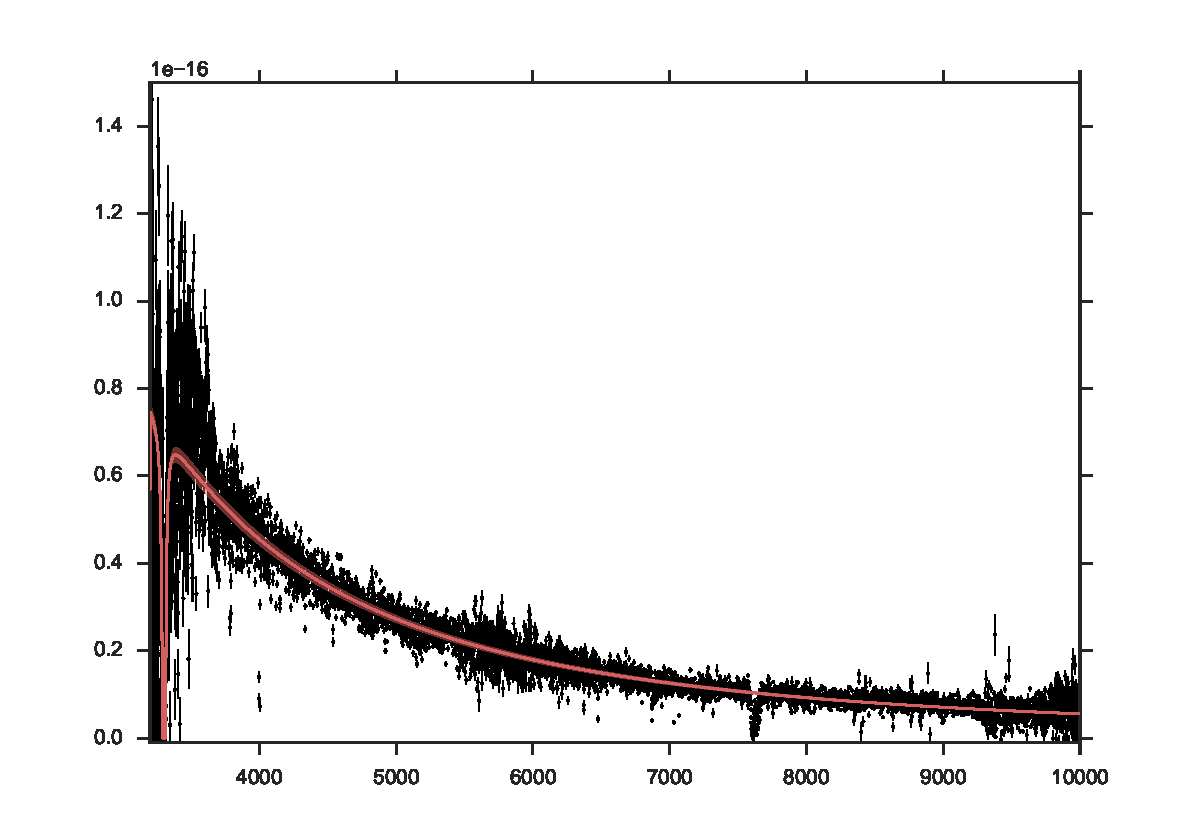
\includegraphics[width=\columnwidth]{figures/DLA_fit.pdf} \caption{The
		voigt-profile fit to the \lya-absorption. The black dots with errorbars is the
		data and associated errors for the spectrum, binned by 10 pixels. The fit is
		performed on the un-binned spectrum. The red line is the fit obtained using the
		median value of the posterior distribution of each of the fit parameters with
		the red shaded area representing the 1-$\sigma$ width of the distribution.}
	\label{fig:example_figure} \end{figure}


\begin{figure} % To include a figure from a file named example.*
	% Allowable file formats are eps or ps if compiling using latex
	% or pdf, png, jpg if compiling using pdflatex
	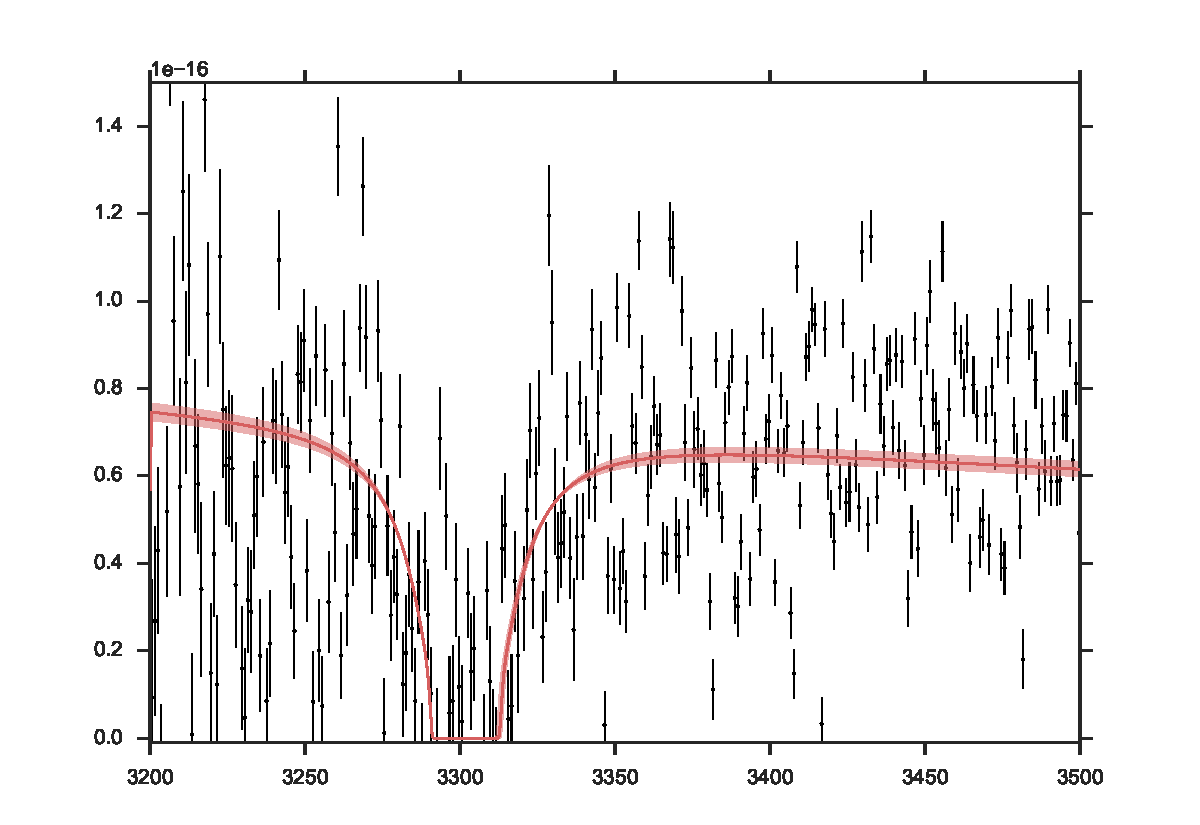
\includegraphics[width=\columnwidth]{figures/DLA_fit_zoom.pdf} \caption{The
		voigt-profile fit to the \lya-absorption. The black dots with errorbars is the
		data and associated errors for the spectrum, binned by 10 pixels. The fit is
		performed on the un-binned spectrum. The red line is the fit obtained using the
		median value of the posterior distribution of each of the fit parameters with
		the red shaded area representing the 1-$\sigma$ width of the distribution.}
	\label{fig:example_figure} \end{figure}



\begin{figure} % To include a figure from a file named example.*
	% Allowable file formats are eps or ps if compiling using latex
	% or pdf, png, jpg if compiling using pdflatex
	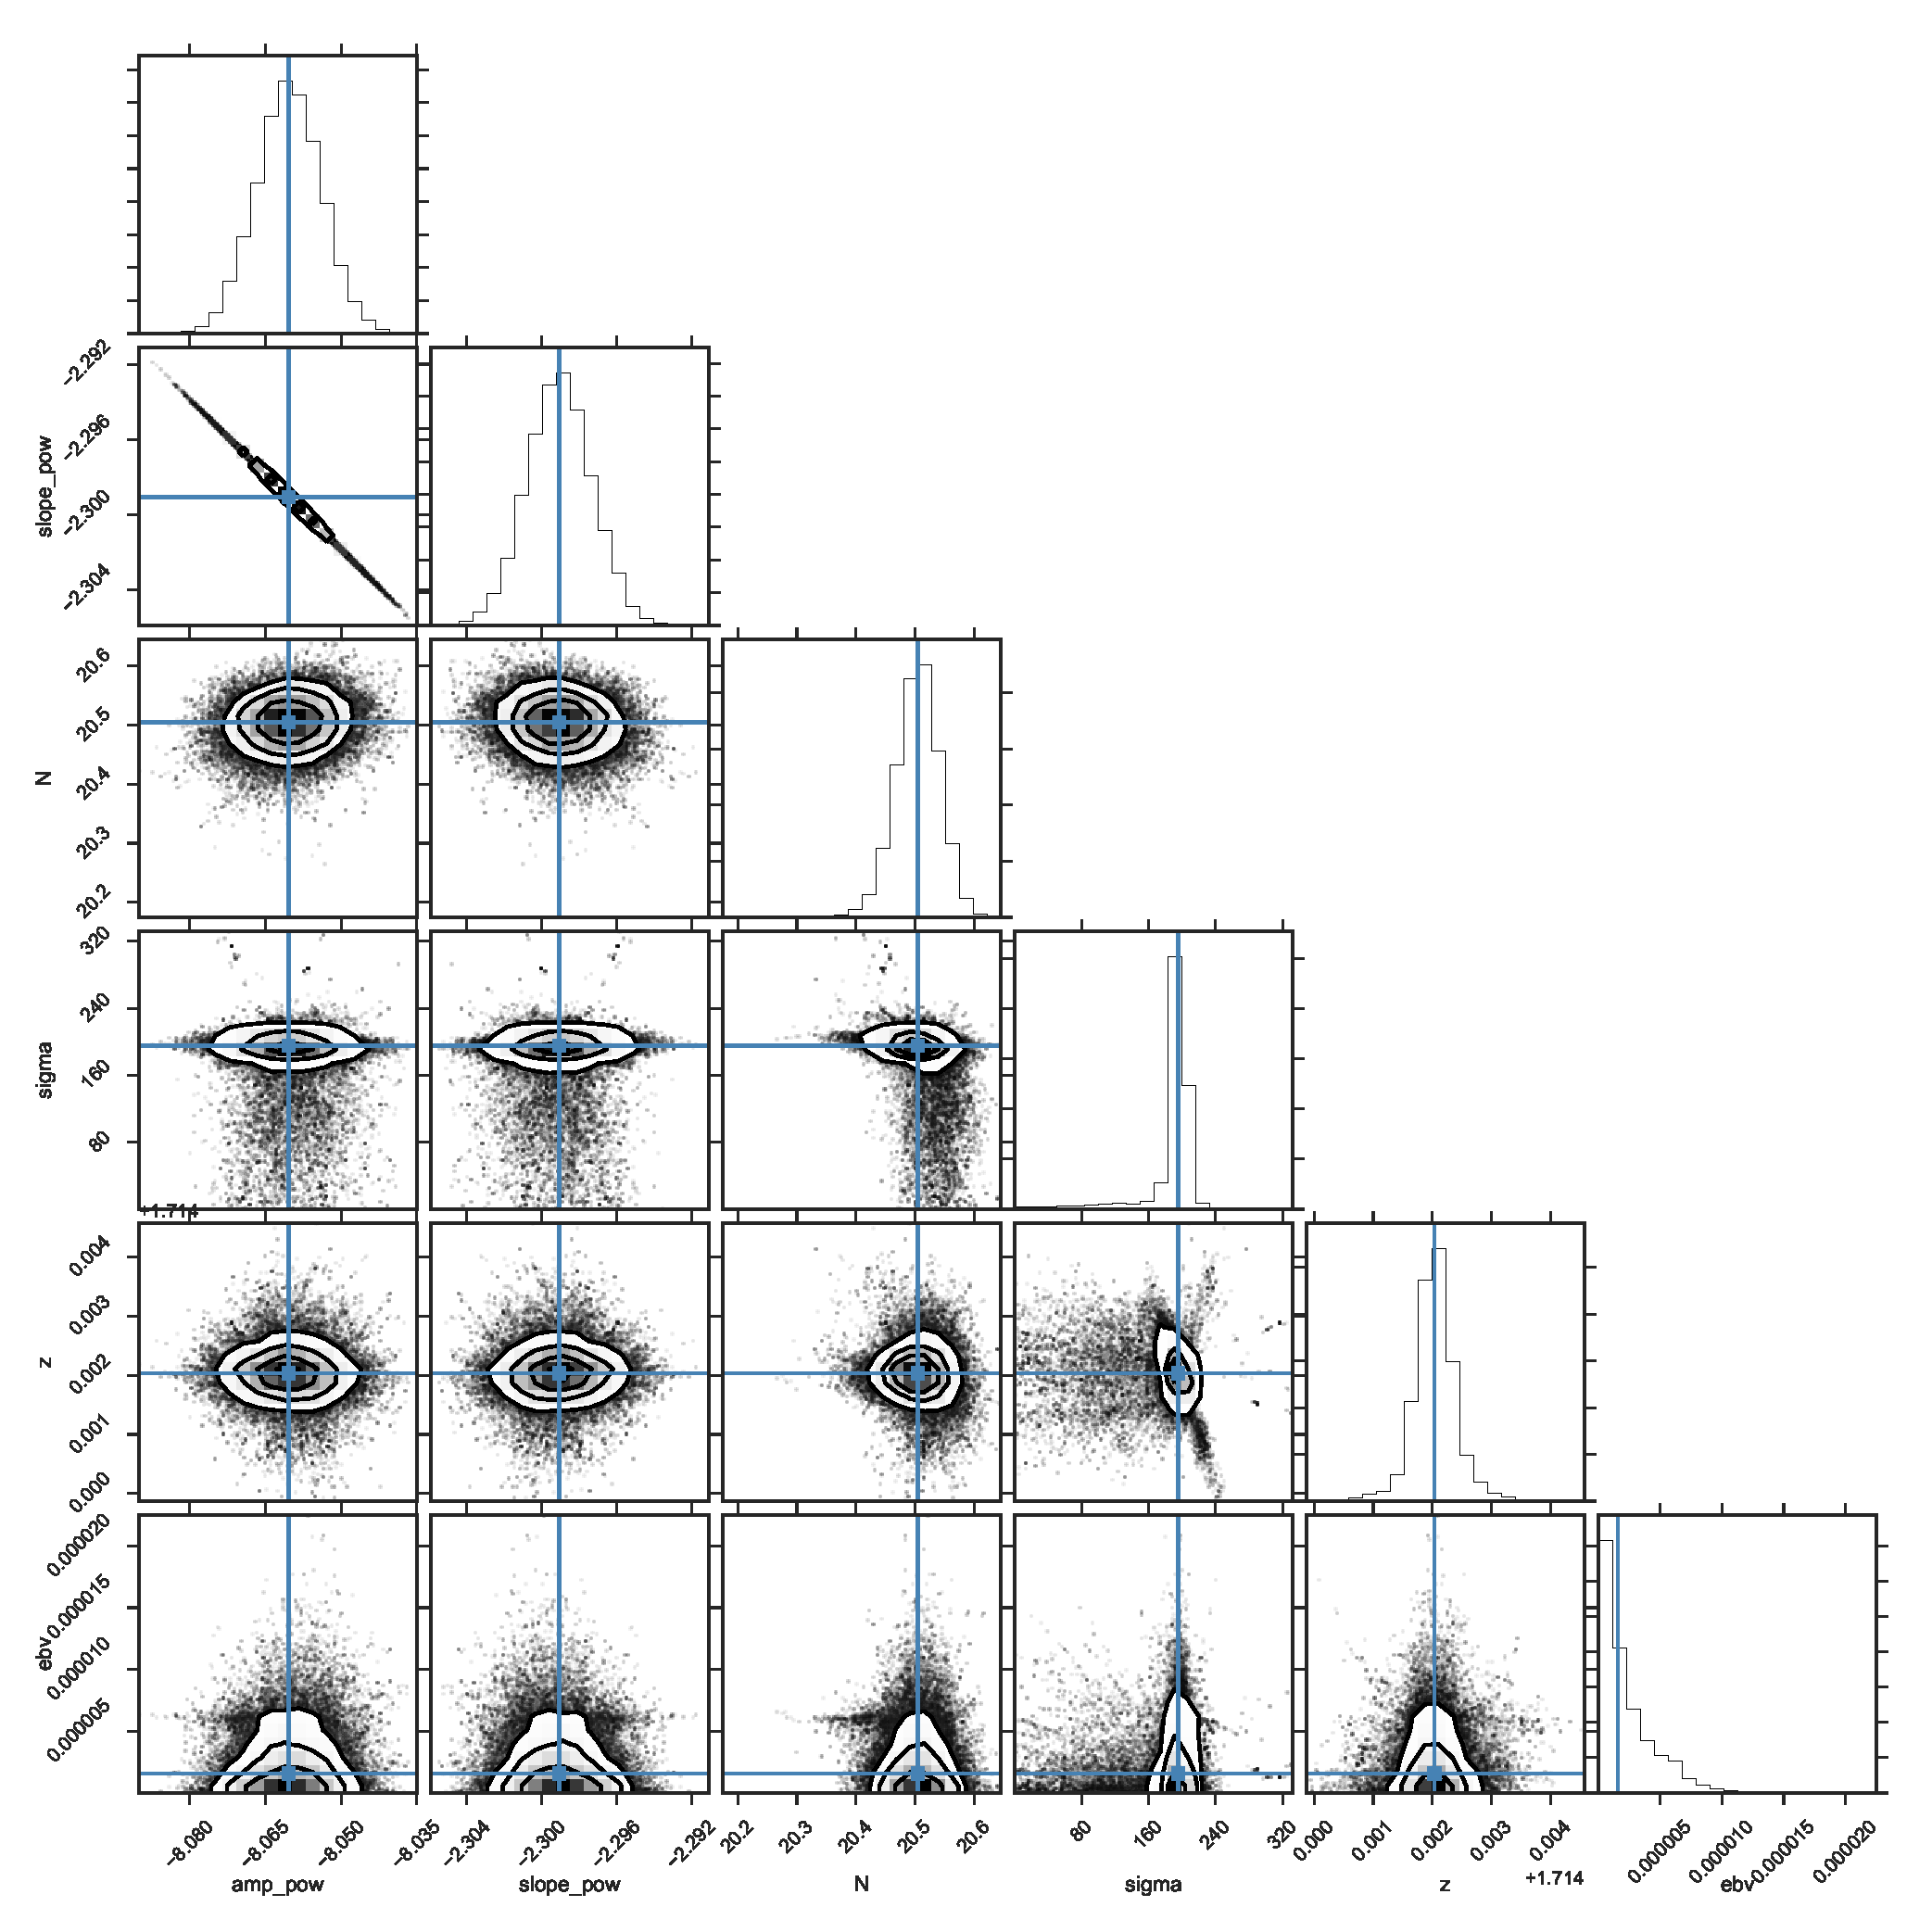
\includegraphics[width=\columnwidth]{figures/Cornerplot.pdf}
	\caption{Cornerplot of the fitted parameters showing the posterior distribution
		of each parameter along with potential correlations. As can be seen the
		continuum slope and amplitude are highly correlated, as expected. The weak
		dependence on the thermal line-broadening is visible from the wide range of
		acceptable values. We give the most likely parameter values as well as their
		credible intervals in \ref{tab:dla_fit} \label{fig:example_figure}}
\end{figure}


\subsection{Line-analysis}


\subsubsection{Kinematic analysis}

\subsubsection{Line-strength analysis}
I did some initial numbers on 160410A, see the table below and the attached
figure. I still need to refine this a bit and calculate some further detection
limits. The lines are quite weak, as compared to the sample that I used in my
paper. I get a LSP of -1.57+/-0.87. This means that the spectrum has features
that are stronger than only 1.6 percent of the sample (or weaker than 98.4
percent). I attach a table with some line detections. We have no detection of
MgII because it falls in the telluric A-band, which is also very strong at the
airmass that we observed.

I'm very surprised that the Keck people see Si II, O I, C IV and Mg II in their
single 600s spectrum. Maybe with a good telluric correction and lower airmass
(they observed at an airmass of 1.05) they can see MgII (there are also minima
at the right locations in our spectra), but I get a 3-sigma limit of $\sim$0.5
\AA~for CIV (0.18 \AA~in rest frame for each of the lines), and there is really
no hint of anything there, nothing. SiII is there and OI could show something at
very low significance, but not CIV. An then they don't see any FeII or AlII that
we do see.

Either they have invented some lines and ignored others, or the spectrum of this
GRB changed a lot during the first hour and a half. I wonder, in that case if
there is any variation between our spectra.

Furthermore, we see no SiIV, which together with the detection of SiII and the
lack of CIV points towards a low ionisation environment. There is no AlIII
either in spite of the AlII, so more to that argument. Line variability may not
be a crazy thought, as we observed really soon, but its still weird. Maybe
someone could find out more about the Keck spectrum? Perhaps they are willing to
contribute to whatever paper comes out of this by providing it (given that what
they claim is real!).

In any case this is a peculiar spectrum with a low column density and low
ionisation environment. There are also no hints of fine structure lines in spite
of the prompt spectrum. I don't know if this means that it is a short GRB, but
it is for sure weird.

\begin{figure}
	% To include a figure from a file named example.*
	% Allowable file formats are eps or ps if compiling using latex
	% or pdf, png, jpg if compiling using pdflatex
	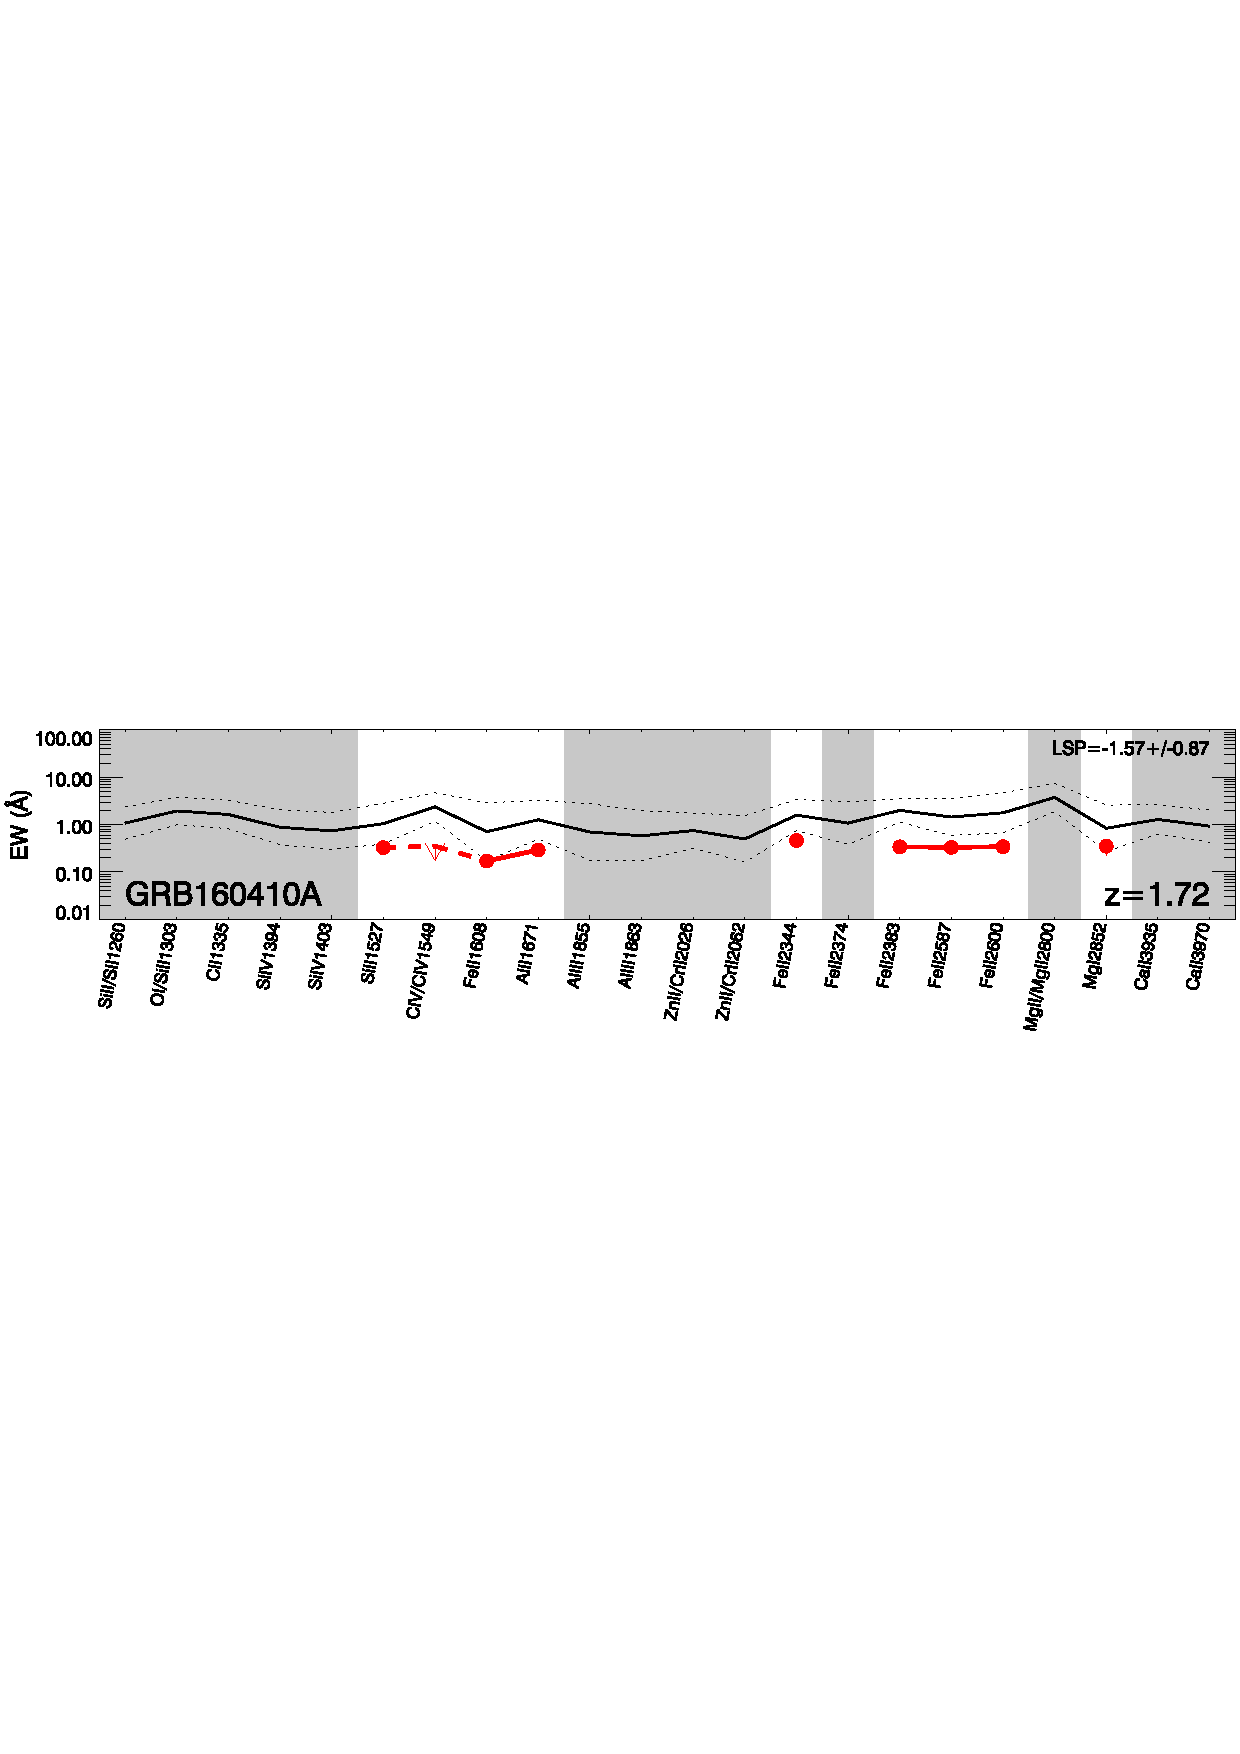
\includegraphics[width=\columnwidth]{figures/160410Alines.pdf}
	\caption{Schematic illustration of the thermal evaporation. \jtodo{Placeholder}}
	\label{fig:example_figure}
\end{figure}


\begin{table*}
\centering
\begin{center}
\caption{Line-strengths inferred.}
% Trigger: 06:47
%\vspace{-0.3cm}
\begin{tabular}{ccccc}
\hline
\noalign{\smallskip}


Wavelength$^{(a)}$& Range             & EW                  &   Feature            & $z$                 \\
({\AA})  & ({\AA})           & ({\AA})             &                      &                     \\
\hline
3406.7 &  3404.3 -  3408.3 &   2.148$\pm$ 0.601  &        SII  1253.520 &  1.71771 ( 1.71760) \\
&                   &                     &         SiIV  1393.8 &  1.44425 ( 1.44450) \\
3784.6 &  3784.0 -  3785.6 &   0.916$\pm$ 0.188  &        CIV  1548.200 &  1.44449 ( 1.44450) \\
3790.6 &  3789.2 -  3791.2 &   0.918$\pm$ 0.212  &        CIV  1550.770 &  1.44430 ( 1.44450) \\
3996.5 &  3995.2 -  3998.4 &   1.548$\pm$ 0.199  &        CIV  1548.200 &  1.58136 ( 1.58150) \\
4003.2 &  4002.0 -  4004.0 &   1.260$\pm$ 0.165  &        CIV  1550.770 &  1.58145 ( 1.58150) \\
4084.1 &  4083.3 -  4084.9 &   0.339$\pm$ 0.137  &       AlII  1670.790 &  1.44443 ( 1.44450) \\
4150.1 &  4148.1 -  4152.5 &   0.890$\pm$ 0.176  &       SiII  1526.710 &  1.71830 ( 1.71760) \\
&                   &                     &         FeII  1608.5 &  1.58016 ( 1.58150) \\
4371.6 &  4370.5 -  4372.5 &   0.463$\pm$ 0.111  &       FeII  1608.450 &  1.71789 ( 1.71760) \\
4540.8 &  4539.3 -  4542.1 &   0.792$\pm$ 0.179  &       AlII  1670.790 &  1.71775 ( 1.71760) \\
\hline
5732.4 &  5730.8 -  5734.8 &   0.853$\pm$ 0.377  &       FeII  2345.000 &  1.44454 ( 1.44450) \\
6371.1 &  6369.7 -  6372.9 &   1.259$\pm$ 0.262  &       FeII  2344.210 &  1.71782 ( 1.71760) \\
&                   &                     &         FeII  2345.0 &  1.71691 ( 1.71760) \\
6475.5 &  6474.1 -  6476.1 &   0.927$\pm$ 0.172  &       FeII  2382.770 &  1.71764 ( 1.71760) \\
7029.5 &  7028.2 -  7030.6 &   0.898$\pm$ 0.158  &       FeII  2586.650 &  1.71762 ( 1.71760) \\
7066.5 &  7065.4 -  7069.0 &   0.932$\pm$ 0.183  &       FeII  2600.170 &  1.71772 ( 1.71760) \\
7753.7 &  7752.4 -  7754.8 &   0.951$\pm$ 0.346  &        MgI  2852.960 &  1.71776 ( 1.71760) \\
9619.0 &  9616.7 -  9620.3 &   0.996$\pm$ 0.345  &       CaII  3934.780 &  1.44461 ( 1.44450) \\


\hline
\hline
\end{tabular}
\end{center}
\noindent{

$^{(a)}$ Blalba .

}
\label{tab:linestrength}

\end{table*}





\section{Environmental census}


\section{Discussion}


\section{Conclusions}



\section*{Acknowledgements}

The Acknowledgements section is not numbered. Here you can thank helpful
colleagues, acknowledge funding agencies, telescopes and facilities used etc.
Try to keep it short.

%%%%%%%%%%%%%%%%%%%%%%%%%%%%%%%%%%%%%%%%%%%%%%%%%%

%%%%%%%%%%%%%%%%%%%% REFERENCES %%%%%%%%%%%%%%%%%%

% The best way to enter references is to use BibTeX:

\bibliographystyle{mnras}
\bibliography{GRB160410A} % if your bibtex file is called example.bib


% Alternatively you could enter them by hand, like this:
% This method is tedious and prone to error if you have lots of references
%\begin{thebibliography}{99}
%\bibitem[\protect\citeauthoryear{Author}{2012}]{Author2012}
%Author A.~N., 2013, Journal of Improbable Astronomy, 1, 1
%\bibitem[\protect\citeauthoryear{Others}{2013}]{Others2013}
%Others S., 2012, Journal of Interesting Stuff, 17, 198
%\end{thebibliography}

%%%%%%%%%%%%%%%%%%%%%%%%%%%%%%%%%%%%%%%%%%%%%%%%%%

%%%%%%%%%%%%%%%%% APPENDICES %%%%%%%%%%%%%%%%%%%%%
\newpage
\appendix

\section{Continuum model}
The optical- and near-infrared continuum of GRB afterglows can be described by a single power law, owing to the continuum generation by syncrotron radiation in the forward shock of the ejected material \citep{Piran2004, Kumar2015},

\begin{equation} 
S_\lambda = S_{0} \lambda^{-\beta},
\end{equation}
where $S_0$ is an arbitrary scaling factor for the flux density and $\beta$ is the power-law slope, both free parameters. 
Additionally, light is attenuated by the presence dust particles which preferentially absorbs shorter wavelength photons, where the detailed dependence is set by the composition of the dust grains. Extinction curves have been parametrized in terms of various shape parameters. We use the parametrization by \citet{Fitzpatrick2007} with the values of SMC-like dust \citep{Gordon2003} for our initial guess, based on the prevalence of SMC-like dust in GRB host galaxies \citep{Japelj2015},

\begin{equation} 
S_\lambda = S_\lambda^*   10 ^{-0.4 E(B-V)[k(\lambda - V) + R_V]},
\end{equation}
where $S_\lambda^*$ is again the unreddened flux value, $E(B-V)$ is the color excess, $R_V$ is the total to selective extinction, meaning how many mangitudes absorption per color excess, and $k(\lambda - V)$ is the wavelength dependent extinction curve,

\begin{equation} 
k(\lambda - V)
\begin{cases}
c_1 + c_2 x + c3 \frac{x^2}{(x - x_0)^2 + x^2 \gamma^2},&  x\leq c_5,\\
c_1 + c_2 x + c3 \frac{x^2}{(x - x_0)^2 + x^2 \gamma^2} + c_4(x - c_5)^2, &  x > c_5,
\end{cases}
\end{equation}
where $x \equiv \lambda^{-1}$ and the rest, $c_1$ through $c_5$ are shape parameters for the extinction curve \citep{Fitzpatrick2007}. 

The continuum level emission will therefore by the product of the intrinsic power-law shape, absorbed by some extinction curve. 



\section{Lyman-$\alpha$ column density} \label{app_absorp}

The background continuum experiences absorption by intervening material, the
strength of which depends on specifics about the absorbing material as well as
the abundance of it. The change in flux observed as the light travels through a
cloud of material is given by the solution to the equation of radiative transfer without emissivity
\begin{equation}
S_\lambda = S_\lambda^* \  e^{ - \sigma_{\lambda} N_j}, 
\end{equation} 
where $S_\lambda^*$ is the incident flux, $S_\lambda$ is the resulting flux,
$\sigma_{\lambda}$ is the wavelength dependent, transition-specific cross
section and $N_j$ is the column density of the absorbable species in state j 
(the state number-density $n_j$ intergrated over the entire line of sight,
$ds$). Therefore the strength of absorption is directly related to the column of
material that we see through. The exponent equals the optical depth,
$\tau_\lambda$, and gives the probability that a photon with a given wavelength
is absorbed. The wavelength-dependent atomic absorbtion cross-section,
$\sigma_{\lambda}$, is composed of two parts; the integrated transition
cross-section, $\sigma_{jk} = \int_{0}^{\infty} \sigma_{\lambda} d\lambda$ for
the transition from state $j$ to state $k$ and the line shape profile $\phi_\lambda$,
which reflects the probability of a photon being absorbed at a given wavelength.
$\sigma_{jk}$ can be calculated from considering the Hamiltonian of the photon -
atom interaction and when disregarding stimulated emission and it is set by the
oscillator strength of the transition, $f_{jk}$, the elementary charge, $e$, and the mass of
the electron, $m_e$, - quantities independent of the environments in which the
absorption takes place,
\begin{equation} 
\sigma_{jk} = \int_{0}^{\infty} \sigma_{\lambda} d\lambda = \frac{\pi  e^2}{m_e c} f_{jk}.
 \end{equation}
Several processes broaden the probability distribution of absorption and
consists of classes, inherently either Lorentzian of Gaussian in shape. The sum
of broadening mechanisms can be parametrized by the convolution of the Gaussian
with the Lorentzian profile, called the Voigt profile ,$V(\lambda, \sigma,
\gamma)$. This profile is specified by the respective widths, $\sigma$ for the
Gaussian and $\gamma$ for the Lorentzian. At the densities considered for the
absorption, the natural line broadening mechanism dominates the Lorentzian width
and is given by $\gamma = \sum\limits_{j<k} A_{jk},$ and is thus specified by
specifics of the transition, leaving only the Gaussian width and the column
density to control the absorption-probability. The absorption signature in a
continuum due to a single atomic transition can thusly be parametrized as

\begin{equation} 
S_\lambda = S_\lambda^* \  e^{ - \frac{\pi  e^2}{m_e c} f_{jk} \lambda_{jk} V(\lambda, \sigma, \gamma)  N_j}, 
\end{equation}
where only $N_j$, and $\sigma$ are free parameters, the rest are specified by the continuum level, $S_\lambda^*$, transition \citep{TepperGarcia2006}.


\section{Likelihood model}

We are interested in exploring the underlying physical parameters that we believe generate our data. In the case of absorption lines, we believe that the column density of the material and the turbulent motion of the gas are the scalar variables that are sufficient to accurately generate the line shape, see \ref{app_absorp}. What we want to quantify is the range of parameter values that, within measurement uncertainties, contain the true physical parameter value. For each spectral point we have for the GRB afterglow, we believe there is an underlying model that can generate that specific data point, $f(\lambda_i, \theta)$, where $\theta$ is the parameters of the model. Following \citet{Hogg2010}, we state a \textit{generative model} for the data, where each data point, $S_{i \lambda}$,  and associated error, $\delta S_{i \lambda}$,  is seen as a normally distributed probability distribution function with the data value being the mean and the y-error, the 1-$\sigma$ width. If we wanted to repeat the measurement, we could resample the entire spectrum where for each point, the value is drawn from the probability distribution function defined by the current measurements. Using our generative model, each data point $(\lambda, S_{i \lambda},\delta S_{i \lambda} )$ has a conditional probability


\begin{equation} 
p(\lambda_i, I(\lambda)_{i} | \theta,  \delta S_{i \lambda})  
=   \frac{1}{\sqrt{2 \pi \delta S_{i \lambda}^2 }}  exp \left(   - \frac{[S_{i \lambda} - f(\lambda, \theta)]^2}{2 \delta S_{i \lambda}^2}    \right),
\end{equation}
where $f(\lambda, \theta)$ is the physical underlying model for the data
\begin{equation} 
f(\lambda, \theta)
=   S_{0} \lambda^{-\beta} \prod_{t=i}^{k} e^{ - \frac{\pi  e^2}{m_e c} f_{t} \lambda_{t} V(\lambda, \sigma, \gamma)  N_t}  10 ^{-0.4 E(B-V)[k(\lambda - V) + R_V]}.
\end{equation}
Here the product is over all absorption lines included in the fit, one component for each transition modeled marked by the subscript, $t$, up to any value $k$. 

\section{The complex error function and the Voigt profile}
As part of the evaluation of the likelihood function we need to evaluate the Voigt-profile. The Voigt profile, which is the convolution of the Gaussian and Lorentzian profiles, can, centered at zero, be written as \citep{pagnini2010} 
\begin{equation} 
	\begin{split}
		V(\lambda,\sigma, \gamma)  
		& = G(\lambda, \sigma)  \otimes L(\lambda, \gamma) \\
		& = \int_{-\infty}^{\infty} G(\xi, \sigma) L(\lambda - \xi, \gamma) d\xi \\
		& = \int_{-\infty}^{\infty} \frac{1}{\sqrt{2 \pi} \sigma} e^{- \left( \frac{\xi}{\sqrt{2} \sigma}  \right)^2 } \frac{1}{\gamma \pi} \frac{\gamma^2}{(\lambda - \xi)^2 + \gamma^2} d\xi \\
		& = \frac{\gamma}{\sqrt{2} \sigma} \frac{1}{ \pi^{3/2}}   \int_{-\infty}^{\infty} \frac{e^{- \left( \frac{\xi}{\sqrt{2} \sigma}  \right)^2 }}{(\lambda - \xi)^2 + \gamma^2}.
	\end{split}
\end{equation}
We can by making the following substitution, $\xi = \sqrt{2} \sigma$ and $d\xi = \sqrt{2} \sigma dt$, write it as
\begin{equation} 
	\begin{split}
		V(\lambda,\sigma, \gamma)  
		& =  \frac{\sqrt{2} \sigma}{ \sqrt{{\pi}}} \frac{\frac{\gamma}{\sqrt{2} \sigma}}{\pi}  \int_{-\infty}^{\infty} \frac{e^{- t^2 }}{(\lambda - \sqrt{2} \sigma t)^2 + \gamma^2} dt \\
		& = \frac{1}{\sqrt{2 \pi} \sigma}  \frac{\frac{\gamma}{\sqrt{2} \sigma}}{\pi}  \int_{-\infty}^{\infty} \frac{e^{- t^2 }}{\left(\frac{\lambda}{\sqrt{2} \sigma} -  t\right)^2 + \left(\frac{\gamma}{\sqrt{2} \sigma}\right)^2} dt.	
	\end{split}
\end{equation}
This form of the convolution is closely related to the complex probability function \citep{letchworth2007, abrarov2015a},
\begin{equation} 
	\begin{split}
		W(z)  
		& = \frac{i}{\pi} \int_{-\infty}^{\infty} \frac{e^{-t^2}}{z - t}  
	\end{split}
\end{equation}
for any complex argument, $z = x + iy$. The complex probability function can be expressed as a sum of a real an imaginary part \citep{benner1995, abrarov2015b},
\begin{equation} 
	\begin{split}
		W(x, y)  
		& = K(x, y) + i L(x, y) \\
		& = \frac{y}{\pi}  \int_{-\infty}^{\infty} \frac{e^{- t^2 }}{(x -  t)^2 +y^2} dt  + \frac{i}{\pi}  \int_{-\infty}^{\infty} \frac{(x - t)e^{- t^2 }}{(x -  t)^2 +y^2} dt,
	\end{split}
\end{equation}
where is the real part, $\mathtt{Re}[W(x, y)] =  \sqrt{2 \pi} \sigma V(\lambda,\sigma, \gamma)$ if $x = \frac{\lambda}{\sqrt{2} \sigma}$ and $y = \frac{\gamma}{\sqrt{2} \sigma}$, which can be obtained by using the complex argument, $z = \frac{\lambda + i\gamma}{\sqrt{2} \sigma}$, in the complex probability function. If $\mathtt{Im}[z] \geq 0$, which is always guaranteed for the width of a spectral profile, the complex probability function equals the complex error function. The complex error function has numerous, fast, numerical approximations where in this work we use the \texttt{scipy.special.wofz} \citep{scipy} implementation.



%%%%%%%%%%%%%%%%%%%%%%%%%%%%%%%%%%%%%%%%%%%%%%%%%%


% Don't change these lines
\bsp	% typesetting comment
\label{lastpage}
\end{document}

% End of mnras_template.tex